% Define some commonly used terms.
% We did include xcolor, didn't we?
\newcommand{\vyse}{\textcolor{blue}{$V_{yse}$ }}
\newcommand{\vmc}{\textcolor{red}{$V_{mc}$ }}
\newcommand{\vxse}{$V_{xse}$ }

\chapter*{Multi Engine Airplanes:\\An Introduction}

Do you want to fly the ``big iron''? Are you looking for more performance, capability,
and reliability? Do you enjoy engine management (and maintenance) so much that you want to
double the fun? If so, the multi engine airplane is for you.

This chapter is meant to prepare the prospective multi engine pilot or instructor for the
fun that is to come.

The material in this section is based upon FAA resources, as well as the Multiengine Manual
that Pilot's Choice Aviation (PCA) in Georgetown, TX distributes to incoming multi engine students.
This document could not exist without Beth Ann Jenkins and Stephanie Fernihough, the authors of the
2017 PCA Multiengine Manual and some notes beyond it.

The Multiengine Manual was reformatted into \LaTeX{} in Spring of 2025. At that time, it was
updated to reflect eight years of students successfully using this document to become multi
engine pilots. It also reflects the latest FAA testing documents as of this writing.

This Manual focused on the Beechcraft Duchess BE76, the primary multi engine trainer used at PCA.

\section*{Disclaimer}

The information contained in this publication is subject to change.

Aeronautical information, regulations, and aircraft information change regularly, therefore those relevant
publications should be referred to for any critical information.

The information in this manual is to be utilized for training purposes only. Always
refer to your aircraft's POH, AFM, and other certified documentation before flight!

\chapter{Single Engine Aerodymanics}

%Keep it above \vyse or bad things happen.
%Keep it above \vmc or really bad things happen.

With a few exceptions, flying a multiengine airplane in normal operations is similar to flying a
complex single. Most of the differences between single-engine and multi-engine flying relate to
emergency situations. Specifically, we are concerned with the airplane’s flight characteristics
when only one engine is fully operating.

The discussion to follow will focus on two key elements of multi-engine flying: performance and controllability.

Note: \emph{performance} and \emph{controllability} are complementary. As one increases, the other decreases, and vice versa.

\section{The Engine-Inoperative Condition}

\subsection{Asymmetric Thrust}

Engines on conventional twins are mounted on the wings. Unlike a single-engine airplane, the engine thrust is not
directed along the longitudinal axis of the airplane. Rather, each engine’s thrust produces a moment that attempts to
yaw the airplane around its vertical axis. On the Duchess (one counter-rotating prop) when both engines are
producing equal thrust, these moments balance each other out and the net thrust has no yawing moment. When one
engine is at reduced or zero thrust, there is a net yawing moment that will lead to a loss of directional control if not
counteracted.

Just like in a single, yawing moments (such as propeller left-turning tendencies in a climb) are counteracted with
rudder. When an engine fails in a multi-engine airplane, the yaw that occurs must be balanced out with enough
rudder pressure to keep the airplane straight. Rudder effectiveness is a function of airspeed – more air flowing over
the rudder airfoil gives it the ability to produce more horizontal lift.

\subsection{Accelerated Slipstream}

Because the engines on a conventional twin are wing-mounted, additional lift is produced by the accelerated
slipstream of the propeller wash over the wing surface. The loss of thrust on one wing results in a loss of lift on that
wing which produces an imbalance of lift between the two wings, leading to a rolling moment toward the
inoperative engine. This rolling tendency must be counteracted with aileron deflection.

\subsection{Summary}

Because of the above listed factors (asymmetric thrust and accelerated slipstream), both produced by the operating
engine, there is a tendency for the airplane to \emph{both} roll \emph{and} yaw into the inoperative engine!

\section{Engine-Inoperative Performance}

\subsection{Loss of Horsepower}

A common misconception is that with one engine out, a twin will have half the climb performance
that it would with both engines. In reality, for aircraft with a maximum gross weight of less than
6,000 pounds, there is no
requirement that they be capable of level flight or climb for \emph{any} weight or flight condition! The only requirement is
that the rate of climb or descent be determined. Many light twins are not capable of holding altitude with one engine.

The Duchess has two 180-HP engines for a total of 360 HP, and requires about 140 HP to maintain level flight.
Losing one engine drastically cuts the horsepower available for climb performance:

\begin{table}[h]
\centering
\begin{tabular}{cl}
\textbf{360}   & \textbf{total HP available}            \\
\textbf{(140)} & \textbf{HP for level flight}           \\ \hline
\textbf{220}   & \textbf{HP left for climb performance} \\
\textbf{(180)} & \textbf{HP -- loss of an engine}       \\ \hline
\textbf{40}    & \textbf{HP now available for climb}
\end{tabular}
\caption{Single engine performance for the Duchess.}
\end{table}

This means we now have only approximately 20\% (40/220) climb performance remaining. In addition,
it should be
stressed that the airplane must be cleaned up to climb. Anything that creates drag will
require additional horsepower
and will decrease the airplane’s climb performance.

Further, realize that 180 HP is the rated horsepower for sea-level standard conditions. Depending on density altitude
(pressure altitude and temperature) effective horsepower may be less than 180 HP. This means that you 
\emph{may not be able to maintain altitude with only one engine}. Maintaining \vyse (blue line) will give you a best rate of climb or the
least rate of descent.

\subsection{\vyse (\textcolor{blue}{Blue Line})}


\vyse is the maximum rate of climb (or minimum rate of sink) airspeed for a single-engine configuration.
It represents
the maximum lift over drag ratio ($L/D_{max}$) with one engine operating, and may be likened to the best glide speed in a
single-engine airplane. At slower airspeeds, induced drag becomes more prominent. At faster speeds, parasite drag
becomes more prominent.

\vyse is the minimum speed to use during all phases of flight and is to be exceeded until committed to land on short
final. \vyse is the minimum speed above which you can commit to a continued takeoff. \vyse is the minimum speed to
use during emergencies involving an engine failure. \vyse is marked by a \textcolor{blue}{Blue Line} on the airspeed indicator (85
KIAS on the Duchess).

\subsection{Drag Factors}

With one engine inoperative, several factors will determine whether or not you'll be able to maintain altitude, climb
or descend. These drag factors increase the horsepower required for level flight, and eat into the excess horsepower
which could be used for climb. All figures are approximate and will vary with density altitude:

\vbox{%
\begin{enumerate}
    \item Not at \vyse -- High or low by 5 knots: \textbf{100 fpm descent}
    \item Gear Down: \textbf{250 fpm descent}
    \item Full Flaps: \textbf{350 fpm descent} (flaps @ 20 = 150 fpm descent)
    \item Critical engine windmilling: \textbf{300 fpm descent}
\end{enumerate}}

Single engine goarounds may be impossible and \textbf{shall not be attempted with flap settings beyond 20 degrees}.

Each twin has a single engine service ceiling and an absolute single engine ceiling:

\begin{itemize}
\item The \textbf{single-engine service ceiling} (Duchess: 6000 ft @ ISA) is the maximum \emph{density altitude} the airplane can sustain a 50 fpm climb with max power on the good engine in the clean configuration.
\item The \textbf{single-engine absolute ceiling} (Duchess: approximately 7800 ft @ ISA) is the maximum \emph{density altitude} the airplane can maintain on one engine with max power in the clean configuration. This is also the altitude where \vyse
and \vxse meet.
\end{itemize}

\subsection{Engine-Inoperative Controllability}

In a single-engine airplane, keeping the aircraft under control (avoiding a stall) is critical. Even if performance is
below that required to maintain level flight, we accept a descent and a controlled landing rather than try to hold off
the descent and get into a stall/spin situation. While stalls are a concern in multi-engine aircraft, another important
consideration is the possible loss of directional control if airspeed is not managed correctly.

With all this in mind, it can be said that the battle for controllability is one between engine and rudder. Anything
that increases the difference in thrust between the two engines will decrease controllability, and anything that makes
the rudder more able to counteract the thrust difference will increase controllability.

\subsection{Critical Engine and Critical Engine Factors}

The critical engine is the engine whose failure most adversely affects the performance and controllability of the
airplane. In general, one of the engines will have a larger yaw moment and the airspeed needs to be higher in order
to balance it out. When the airplane has counter-rotating props (such as the Duchess) there is no critical engine. On
most twins, both propellers rotate clockwise when viewed from the cockpit. On these aircraft, the left engine is
critical. The reasons for this are explained below.

The following discussion assumes a conventional light twin, with two clockwise-rotating propellers. On such
airplanes, the critical engine is the left engine, because the left-turning tendencies of the right engine add to its
asymmetric thrust. The left turning tendencies are discussed below. (PAST)

\subsubsection{P factor}

The descending blade produces more thrust than the ascending blade. The descending blade on the right engine has
a longer moment arm (A2) than on the left engine (A1). This produces greater asymmetric thrust when the right
engine is operating than when the left engine is operating.

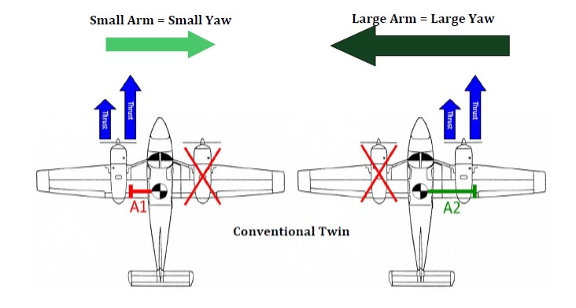
\includegraphics[width=\linewidth]{pfactor}
